\documentclass[11pt,a4paper]{report}
\usepackage[portuges]{babel}
\usepackage[utf8]{inputenc} 
\usepackage{graphicx} 
\usepackage{url} 
\usepackage{enumerate} 
\usepackage{color} 
\usepackage{textcomp}
\usepackage{indentfirst}
\usepackage{array} 
\usepackage{parskip}
\usepackage[export]{adjustbox}
\usepackage{xpatch}
\usepackage{amsmath}
\newlength{\chaptertopskip}
\setlength{\chaptertopskip}{10pt}

\usepackage{a4wide}
\usepackage{float}
\usepackage{minted}
\usepackage{multicol}
\usepackage{appendix}
\setlength{\parskip}{1em}
\usepackage{verbatim}

\usepackage[demo]{graphicx}
\usepackage{caption}
\usepackage{subcaption}


\usepackage[pdftex]{hyperref} % transformar as referências internas do seu documento em hiper-ligações.

\definecolor{saddlebrown}{rgb}{0.55, 0.27, 0.07} % para definir uma nova cor, neste caso 'saddlebrown'

\usepackage{listings}  % para utilizar blocos de texto verbatim no estilo 'listings'
%paramerização mais vulgar dos blocos LISTING - GENERAL
\lstset{
	basicstyle=\small, %o tamanho das fontes que são usadas para o código
	numbers=left, % onde colocar a numeração da linha
	numberstyle=\tiny, %o tamanho das fontes que são usadas para a numeração da linha
	numbersep=5pt, %distancia entre a numeração da linha e o codigo
	breaklines=true, %define quebra automática de linha
    frame=tB,  % caixa a volta do codigo
	mathescape=true, %habilita o modo matemático
	escapeinside={(*@}{@*)} % se escrever isto  aceita tudo o que esta dentro das marcas e nao altera
}

\usepackage{xspace} % deteta se a seguir a palavra tem uma palavra ou um sinal de pontuaçao se tiver uma palavra da espaço, se for um sinal de pontuaçao nao da espaço

\parindent=20pt %espaço a deixar para fazer a  indentação da primeira linha após um parágrafo
\parskip=10pt % espaço entre o parágrafo e o texto anterior

\setlength{\oddsidemargin}{-1cm} %espaço entre o texto e a margem
\setlength{\textwidth}{18cm} %Comprimento do texto na pagina
\setlength{\headsep}{0cm} %espaço entre o texto e o cabeçalho
\setlength{\textheight}{23cm} %altura do texto na pagina
\renewcommand{\baselinestretch}{1.5cm}


\begin{document}
\begin{figure}
    
\includegraphics[scale=0.3]{logoum.png}
\end{figure}
\title{\textbf{Transformações Geométricas}\\
       \textbf{Unidade Curricular de Computação Gráfica}\\ Licenciatura em Ciências da Computação\\Universidade do Minho
       } %Titulo do documento
\author{Bruno Jardim\\ (A91680) \and Inês Presa\\ (A90355)
         \and Tiago Carriço\\ (A91695) \and Tiago Leite\\ (A91693)
       } %autores do documento
\date{\today} %data
\maketitle
\begingroup
\renewcommand*\contentsname{Índice}
\let\clearpage\relax
\tableofcontents


\endgroup
\newpage

\chapter{Contextualização}    
No âmbito da unidade curricular de Computação Gráfica da Licenciatura em Ciências da Computação foi proposta o desenvolvimento em \textit{Opengl} de um motor gráfico genérico que terá como função a criação de um sistema solar. Desenvolvimento esse que deve ser composto por quatro etapas. 

\section{Enunciado}
Nesta terceira etapa foi proposto:

\begin{itemize}
    \item \textbf{Desenho de superfícies de Bezier}
        \begin{description}
        \item Alteração do \textit{generator} de modo a ler ficheiros com \textit{patches} de Bezier e pontos de controlo e retornar a lista de triângulos necessários para desenhar a suprefície, de acordo com o nível de tesselação requerido. 
        \end{description}

    \item \textbf{Extensão das translações e rotações}
    \begin{description}
    \item As translações devem poder ser constituídas por um conjunto de pontos de controlo, que definam uma curva de Catmul-Rom por onde o modelo sobre o qual é aplicada a transformação se vai mover, assim como o número de segundos que este demora a descrever a curva.
    \item Nas rotações, o ângulo deve poder ser substituído pelo tempo que o modelo demora a girar sobre si próprio. 
    \end{description}
    
   
    
    \item \textbf{Modelo dinâmico do sistema solar}
    \begin{description}
    \item Alterar o ficheiro de configuração XML de modo a criar um modelo dinâmico do sistema solar.
    \end{description}
    
    \item \textbf{VBOs}
    \begin{description}
    \item Os modelos escolhidos no ficheiro de configuração XML, devem ser armazenados e  desenhados com recurso a VBOs. 
    \end{description}
\end{itemize}


\chapter{Apresentação das soluções}
\section{Desenho de superfícies de Bezier}
Para o desenho de suprefícies de Bezier, alterou-se o \textit{generetor} de modo a que fosse possível ler um ficheiro com várias \textit{patches} e pontos de controlo e criar um ficheiro .3d com o conjunto de pontos necessários para o desenho da superfície, de acordo com o nível de tesselação. Assim sendo, para além do tipo de modelo, o \textit{generator} recebe como parâmetros:
\begin{itemize}
    \item o ficheiro \textit{input} com as \textit{patches} e pontos de controlo.
    \item o nível de tesselação.
    \item o ficheiro de \textit{output}.
\end{itemize}
Para a obtenção dos pontos necessários à construção de cada superfície foi utilizada a seguinte fórmula:
\par
Seja a matriz de Bezier \emph{M =}
\begin{bmatrix}
-1 & 3 & -3 & 1\\
3 & -6 & 3 & 0\\
-3 & 3 & 0 & 0\\
1 & 0 & 0 & 0
\end{bmatrix}
\par
\emph{T =} nível de tesselação
\par
4 curvas de Bezier \emph{$C_0$,$C_1$,$C_2$,$C_3$}
\par
\emph{$C_0 = P_{00} , P_{10} , P_{20} , P_{30}$}
\par
\emph{$C_1 = P_{01} , P_{11} , P_{21} , P_{31}$}
\par
\emph{$C_2 = P_{02} , P_{12} , P_{22} , P_{32}$}
\par
\emph{$C_3 = P_{03} , P_{13} , P_{23} , P_{33}$}
\par
\emph{$B(u,v) =$}
\begin{bmatrix}
\emph{$u^3$} & \emph{$u^2$} & \emph{$u$} & \emph{$1$}\\
\end{bmatrix}
\emph{$M$}
\begin{bmatrix}
\emph{$P_{00}$} & \emph{$P_{01}$} & \emph{$P_{02}$} & \emph{$P_{03}$}\\
\emph{$P_{10}$} & \emph{$P_{11}$} & \emph{$P_{12}$} & \emph{$P_{13}$}\\
\emph{$P_{20}$} & \emph{$P_{21}$} & \emph{$P_{22}$} & \emph{$P_{23}$}\\
\emph{$P_{30}$} & \emph{$P_{31}$} & \emph{$P_{32}$} & \emph{$P_{33}$}
\end{bmatrix} 
\emph{$M^T$}
\begin{bmatrix}
\emph{$v^3$}\\
\emph{$v^2$}\\
\emph{$v$} \\
\emph{$1$} 
\end{bmatrix}
\par
Os vários pontos da superfície são obtidos utilizando a função \emph{B} variando \emph{u} e \emph{v} entre 0 e 1.
\par
Por exemplo com:
\par
\emph{a = B(0,0) b = B(1/T,0) c = B(1/T,1/T) d = B(0,1/T)}
\par
Pode-se construir os triângulos \emph{a,b,d} e \emph{b,c,d}. 

\subsection{Superfícies geradas}

\vspace{1cm}
\begin{figure}[H]
\centering
\begin{subfigure}{0.5\textwidth}
  \centering
  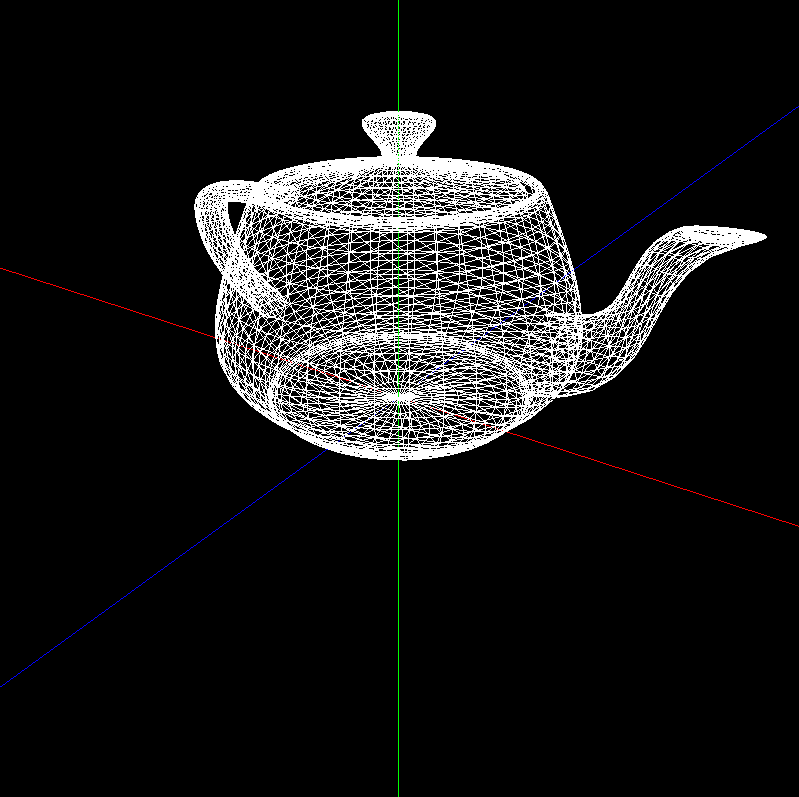
\includegraphics[width = 8cm,height = 8cm]{teapot_tesselation_10.png}
  \caption{\texttt{teapot com tesselação 10}}
  \label{fig:teapot com tesselação 10}
\end{subfigure}%
\begin{subfigure}{0.5\textwidth}
  \centering
  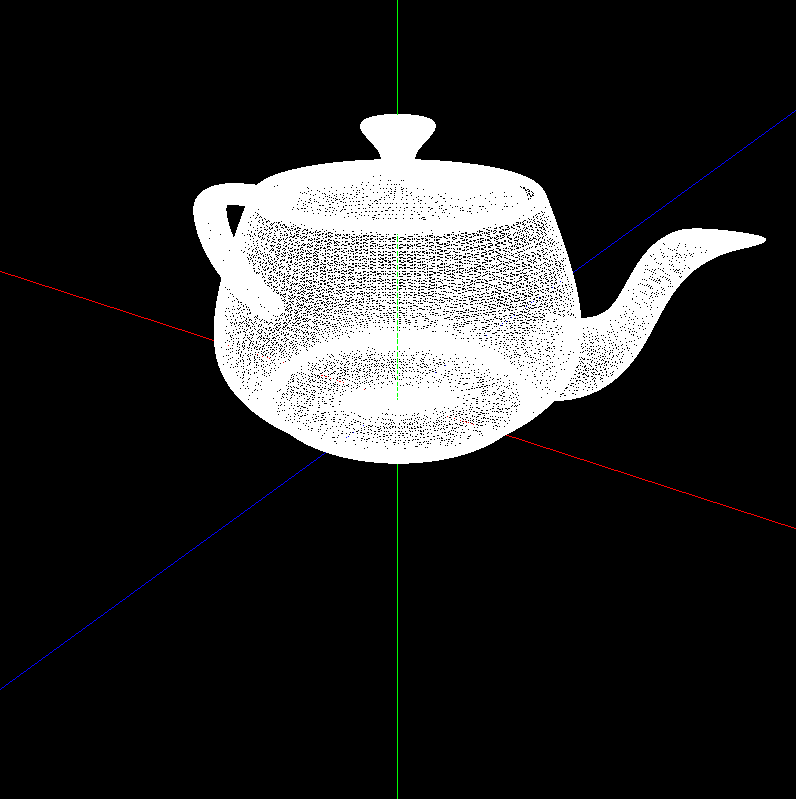
\includegraphics[width = 8cm,height = 8cm]{teapot_tesselation_30.png}
  \caption{\texttt{teapot com tesselação 30}}
  \label{fig:teapot com tesselação 30}
\end{subfigure}
\label{fig:teapots}
\caption{Execução do \textit{engine} com os pontos gerados através do ficheiro de \textit{patches}}
\end{figure}


\newpage
\section{Extensão das translações e rotações}
Fizeram-se alterações quanto às translações e rotações de forma a que estas fossem capazes de, no caso das translações fazê-las sobre uma curva de Catmull-Rom, e no caso das rotações fazer com que estas funcionassem em função do tempo, para além de um ângulo tal como estava implementado previamente.



\subsection{Demonstração}

\vspace{1cm}
\begin{figure}[H]
\centering
\begin{subfigure}{0.5\textwidth}
  \centering
  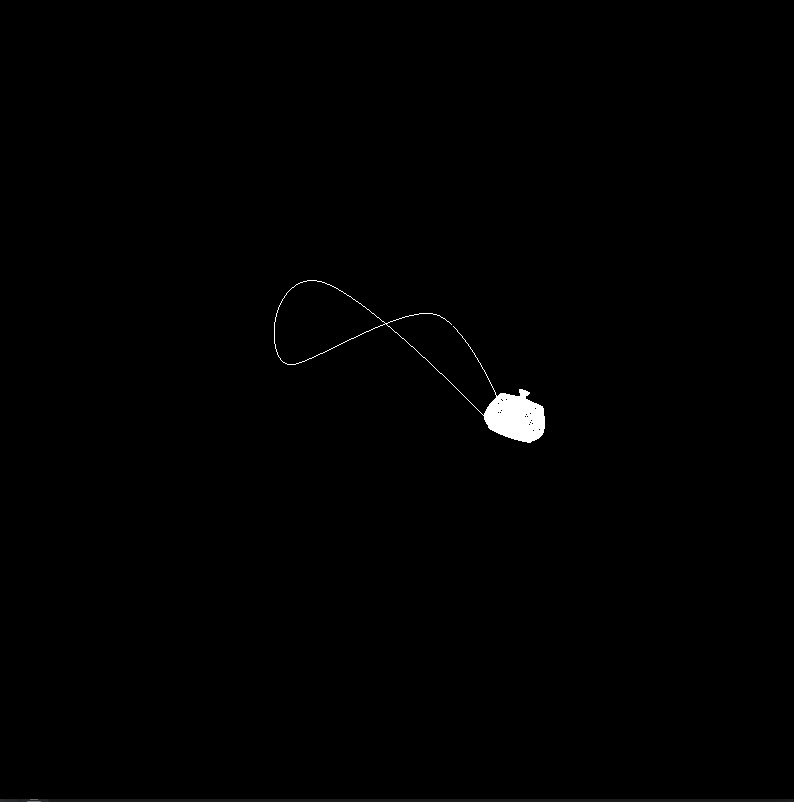
\includegraphics[width = 8cm,height = 8cm]{catmul_teapot1.png}
  \caption{\texttt{}}
  \label{fig:catmul_teapot1}
\end{subfigure}%
\begin{subfigure}{0.5\textwidth}
  \centering
  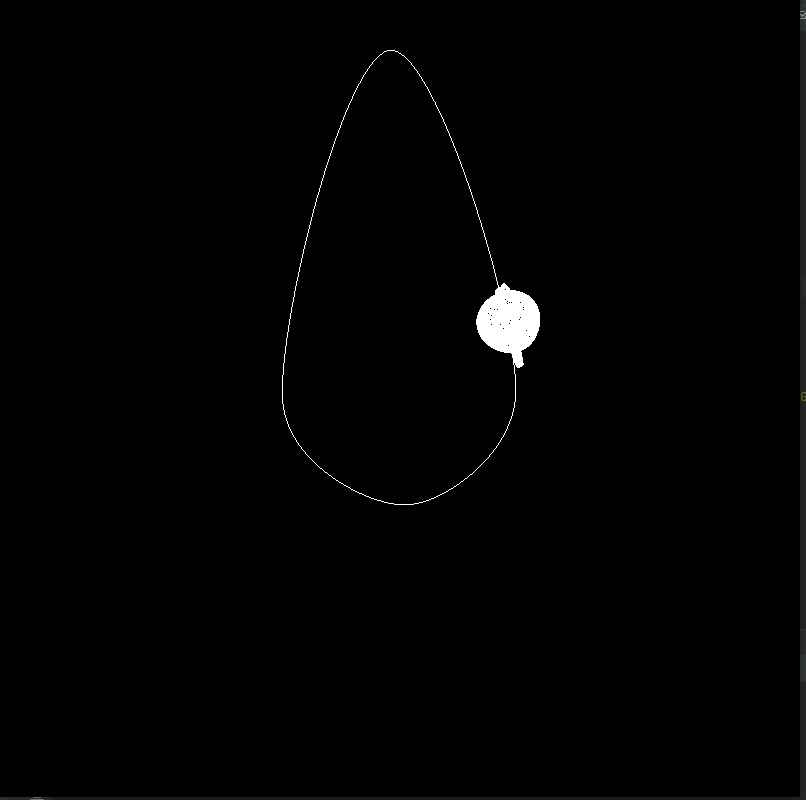
\includegraphics[width = 8cm,height = 8cm]{catmul_teapot2.png}
  \caption{\texttt{}}
  \label{fig:catmul_teapot1}
\end{subfigure}
\begin{subfigure}{0.5\textwidth}
  \centering
  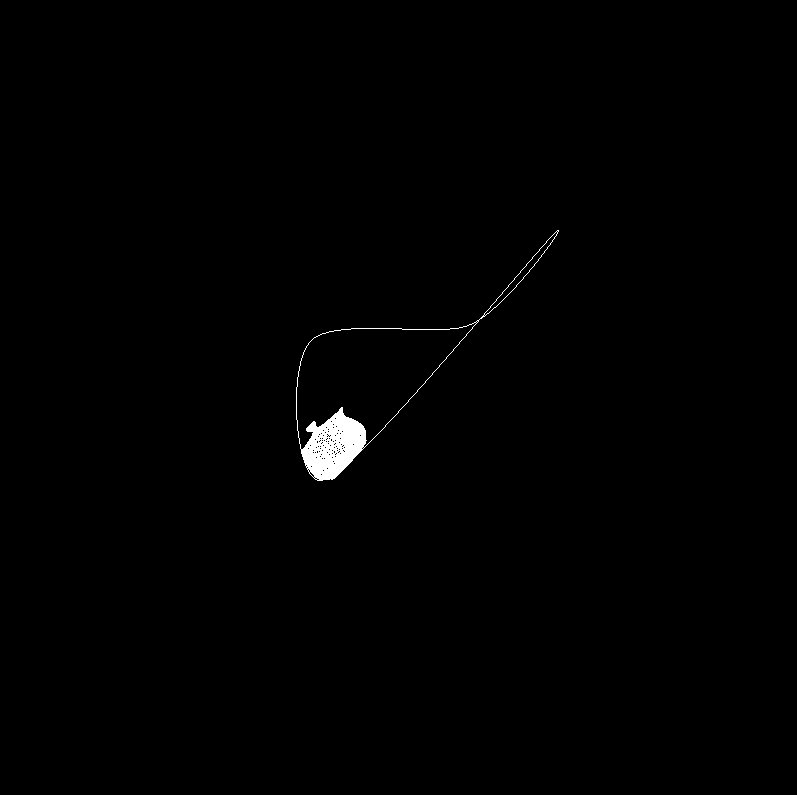
\includegraphics[width = 8cm,height = 8cm]{catmul_teapot3.png}
  \caption{\texttt{}}
  \label{fig:catmul_teapot1}
\end{subfigure}%
\begin{subfigure}{0.5\textwidth}
  \centering
  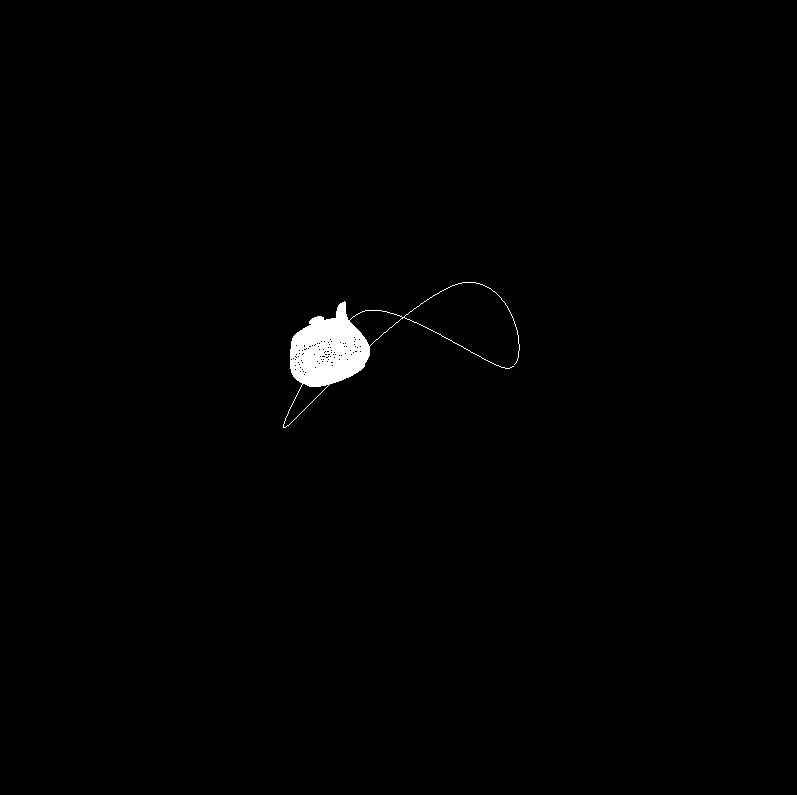
\includegraphics[width = 8cm,height = 8cm]{catmul_teapot4.png}
  \caption{\texttt{}}
  \label{fig:catmul_teapot1}
\end{subfigure}
\label{fig:teapots}
\caption{Teapot gerado pelo  \textit{patch} a descrever curva de Catmul-Rom}
\end{figure}

\newpage

\section{Modelo dinâmico do sistema solar}
Para construir as órbitas dos planetas foram utilizados 8 pontos de controlo de modo a criar as curvas de Catmull-Rom. Assim sendo, utilizou-se a distância dos planetas ao Sol que já tinha sido calculada na fase anterior e procedeu-se da seguinte forma:
\par
Seja  D a distância do planeta ao sol, $F = \sqrt{2}/2 \ e \ {p_0},\ {p_1},\ {p_2},\ {p_3},\ {p_4},\ {p_5},\ {p_6},\ {p_7}$ \ pontos \ de \ controlo, temos:
\par
{$p_0 = (F \times D, \ 0,\ F \times D)$}
\par
{$p_1 = (0, \ 0, \ D)$}
\par
{$p_2 = (- \ F \times D,\ 0,\ F \times D)$}
\par
{$p_3 = (- \ D,\ 0,\ 0)$}
\par
{$p_4 = (- \ F \times D,\ 0, - \ F \times D)$}
\par
{$p_5 = (F \times 0,\ 0, - \ D)$}
\par
{$p_6 = (F \times D,\ 0, - \ F \times D)$}
\par
{$p_7 = (D,\ 0,\ 0)$}





\subsection{Demonstração}

\vspace{1cm}
\begin{figure}[H]
\centering
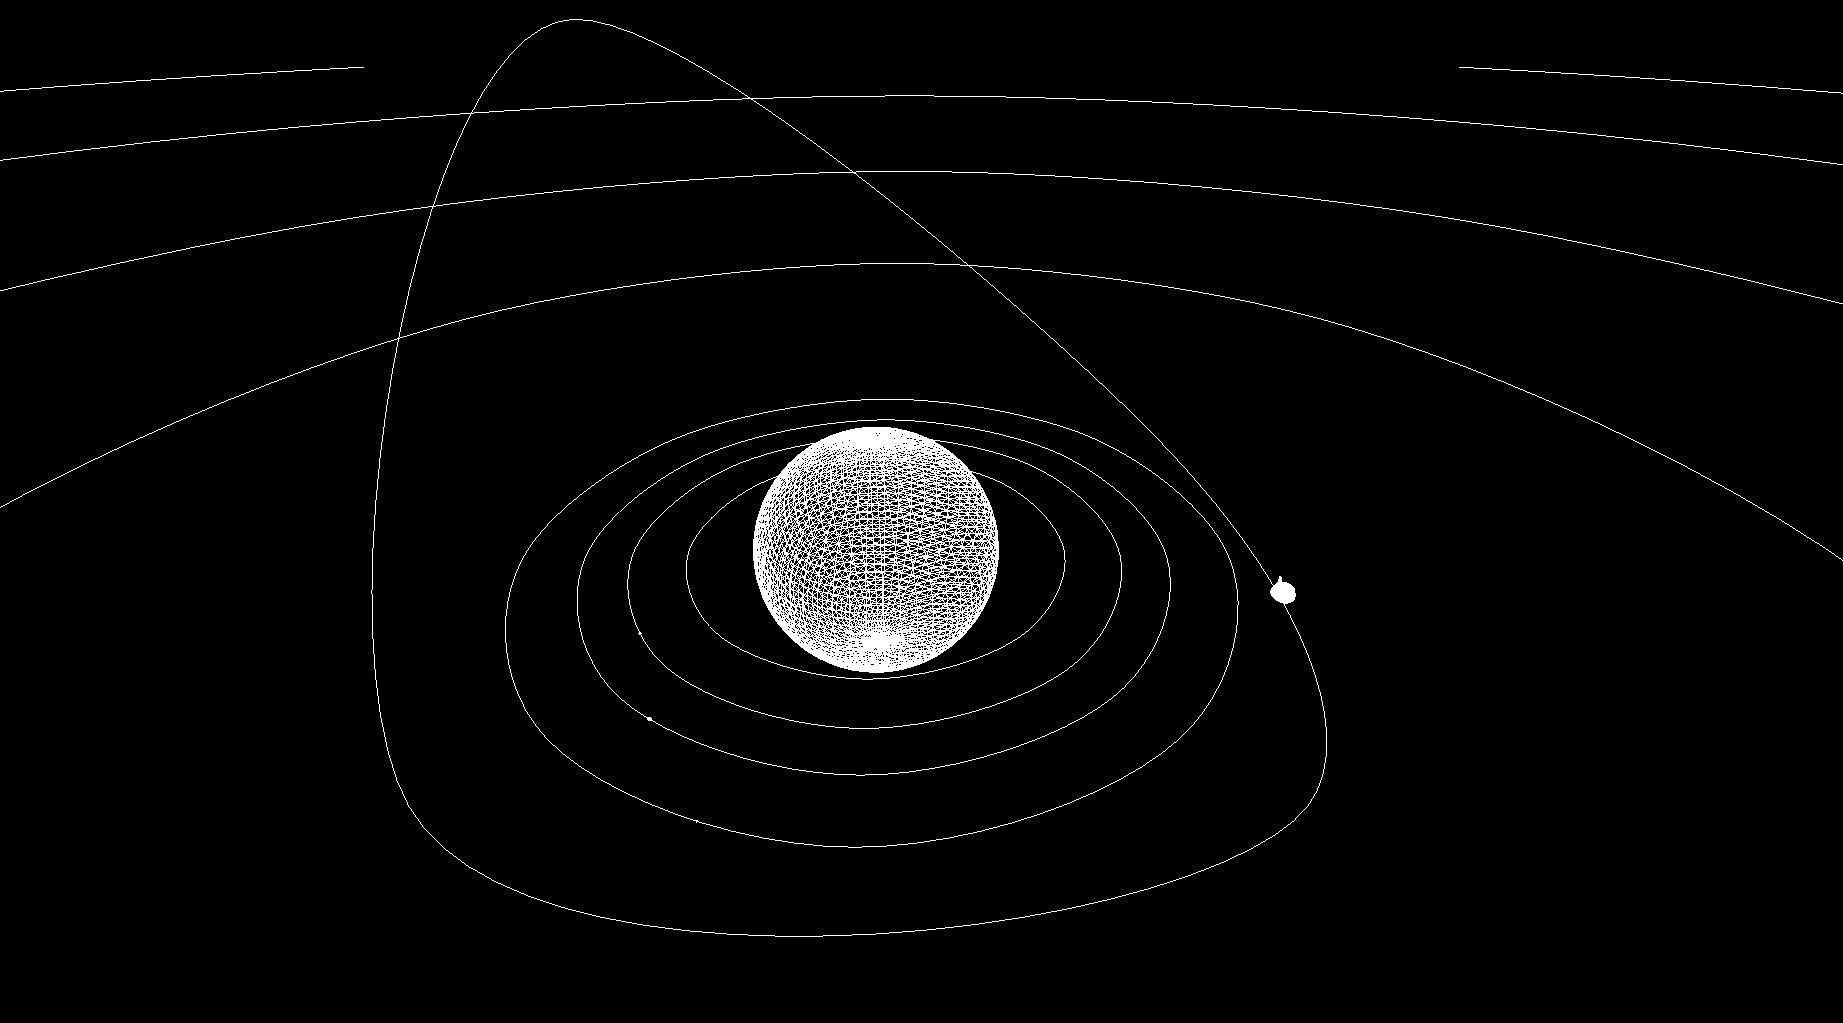
\includegraphics[width = 18cm,height = 10cm]{ss1.png}
\caption{Vista global}
\label{fig:demo1}
\end{figure}

\begin{figure}[H]
\centering
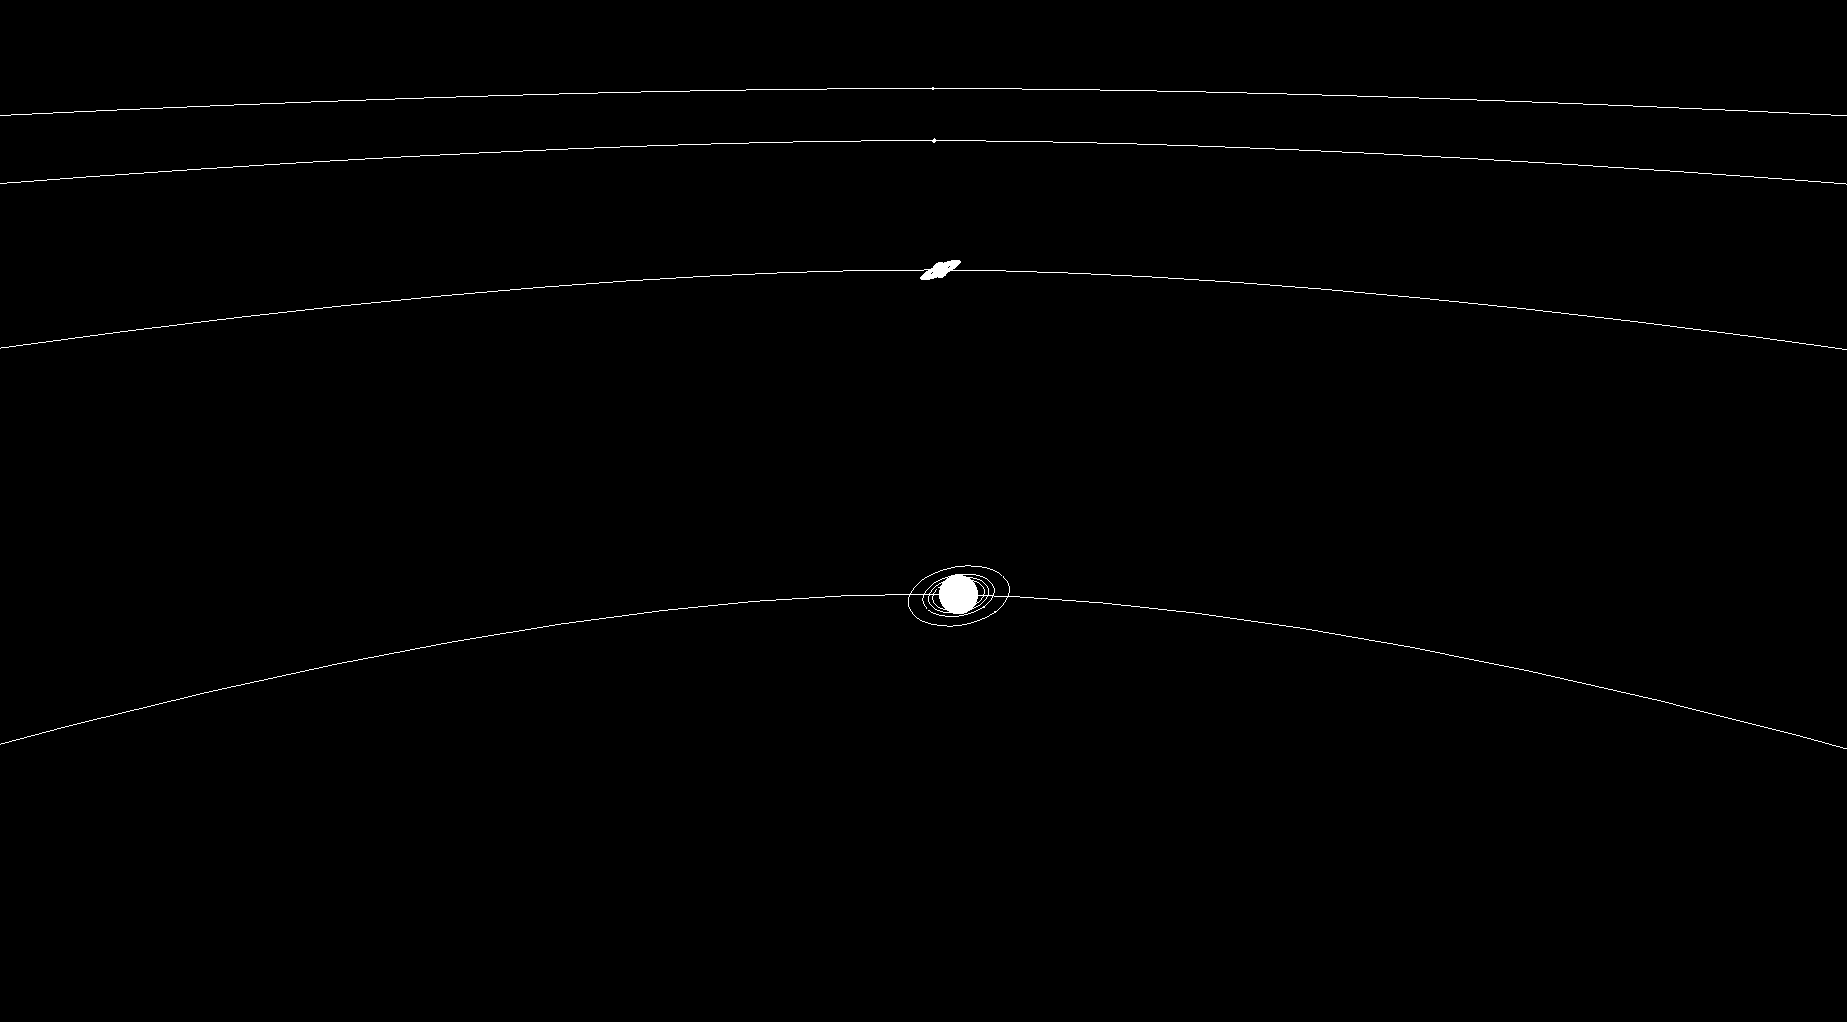
\includegraphics[width = 18cm,height = 10cm]{ss2.png}
\caption{Júpiter - Saturno}
\label{fig:demo2}
\end{figure}

\begin{figure}[H]
\centering
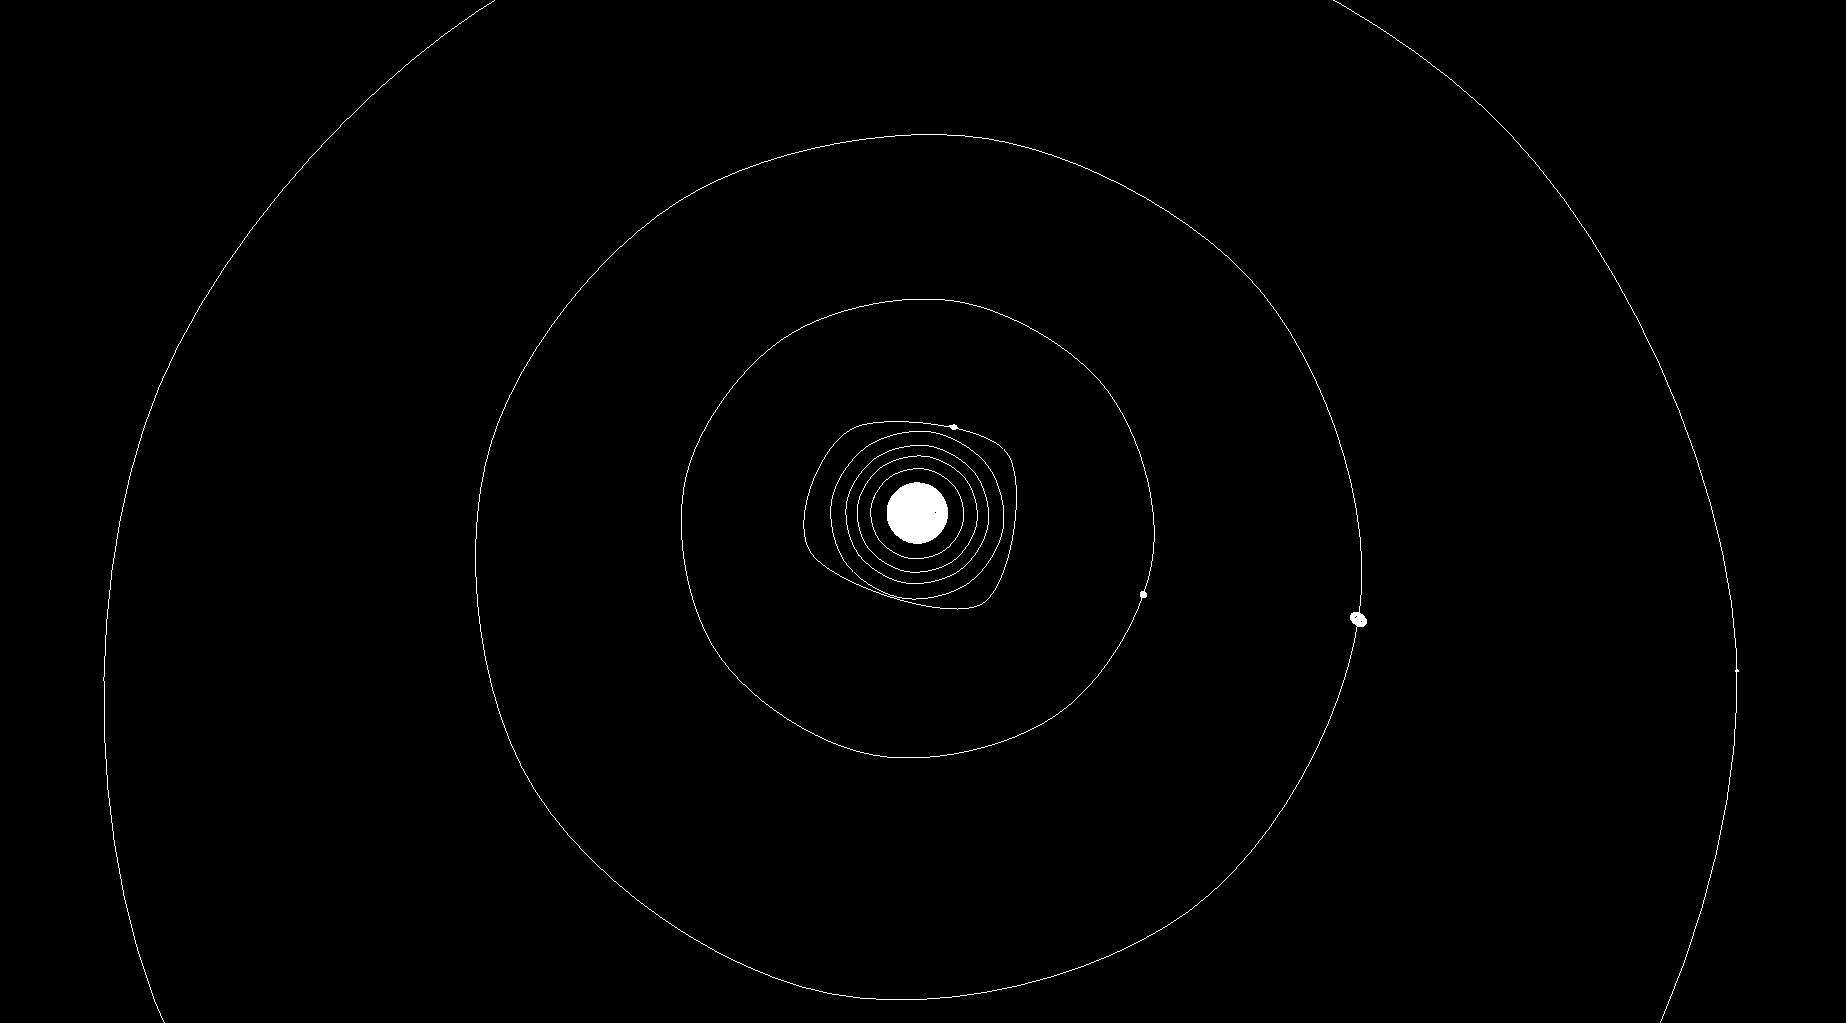
\includegraphics[width = 18cm,height = 10cm]{ss3.png}
\caption{Vista superior}
\label{fig:demo3}
\end{figure}

\begin{figure}[H]
\centering
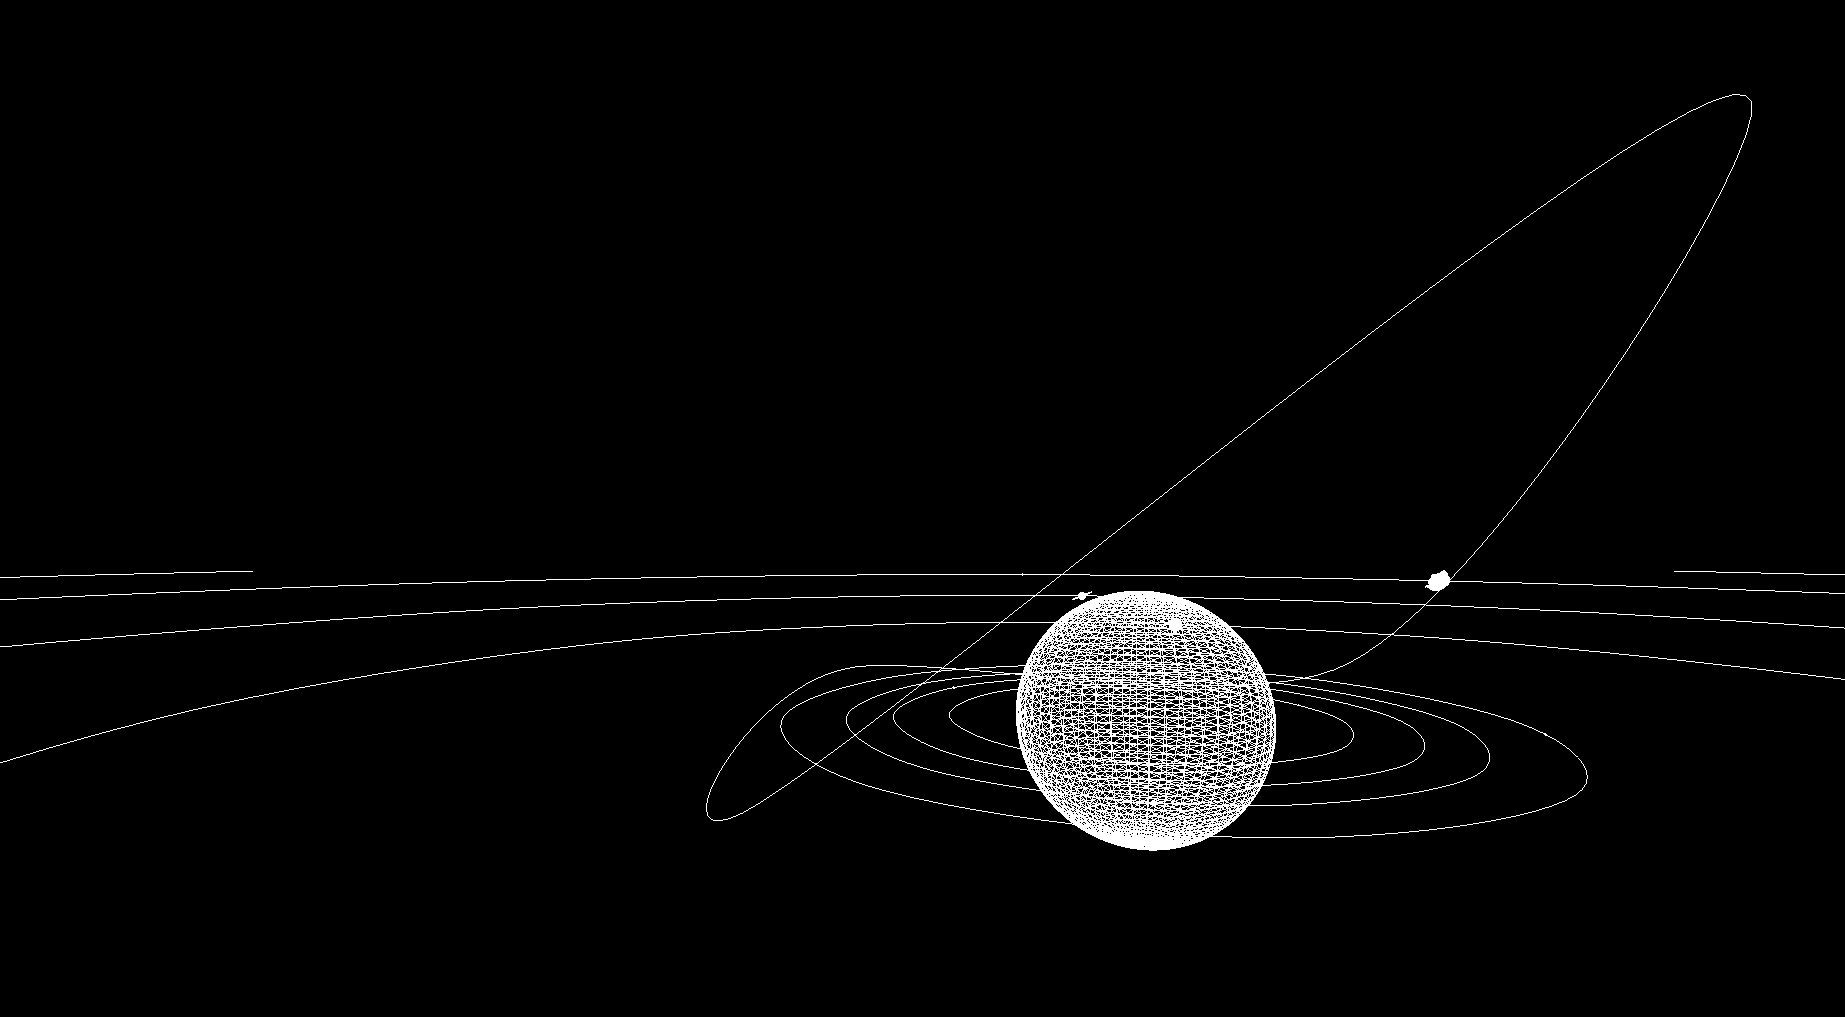
\includegraphics[width = 18cm,height = 10cm]{ss4.png}
\caption{Órbita do cometa}
\label{fig:demo4}
\end{figure}




\section{VBOs}
Na implementação dos VBOs optou-se por utilizar um VBO para cada figura, pois pareceu ser a solução mais simples. No entanto, cada modelo diferente possui um só VBO. Por exemplo, se existirem várias esferas iguais, apenas é utilizado um VBO para todas.

\newpage


\newpage
\chapter{Conclusão}
No início da construção da solução chegou-se ao consenso de que a funcionalidade mais complexa de se implementar seria a dos VBO's, dado isto, o grupo tomou a decisão de que esta seria a última a ser implementada. Para além da sua complexidade, outro motivo para esta decisão foi que estes teriam influência sobre todo o projeto, ao contrário das outras funcionalidades, desta forma foi possível implementar e testar as outras funcionalidades com a certeza de que qualquer erro que surgisse não era devido a erros na implementação dos VBO's.

Dado isto considera-se que foi um trabalho bem conseguido e que se atingiu os objetivos propostos.


\end{document}
